\chapter{Interfața utilizatorului și experiența de utilizare}

Acest capitol descrie modul în care funcționalitățile implementate sunt prezentate utilizatorului prin interfața web. Dacă în capitolul anterior am detaliat deciziile tehnice din spatele fiecărei componente, acum mă concentrez pe experiența concretă: cum navighează un utilizator prin aplicație, ce funcții sunt disponibile pentru fiecare rol și cum contribuie deciziile de interfață la o utilizare naturală și eficientă a platformei.

Interfața WhereWeFishin este o aplicație Angular de tip SPA, cu rutare lazy și componente standalone. Structura sa urmărește separarea clară a rolurilor: fiecare categorie de utilizator are zone proprii, accesibile prin rute protejate și cu un set delimitat de funcții disponibile. Separarea nu este doar de securitate, ci și de claritate: utilizatorul obișnuit nu vede funcțiile administrative, iar managerul nu este expus la zona de supraveghere a administratorului.

\section{Principii de organizare a interfeței}

Proiectarea interfeței a pornit de la câteva constrângeri clare. Aplicația trebuie să fie utilizabilă de persoane fără experiență tehnică, mai precis pescari care caută un loc de pescuit și vor să facă o rezervare cât mai simplu posibil. Totodată, trebuie să ofere un panou de control util pentru manageri, care au nevoie de acces rapid la informații operaționale. Ambele cerințe trebuie satisfăcute de aceeași aplicație, ceea ce impune o separare clară a zonelor și o navigare intuitivă.

Structura generală urmează o ierarhie de trei niveluri. La primul nivel se află zonele mari ale aplicației: zona publică (hartă și detalii locații), zona utilizatorului autentificat (rezervări, analiză media, profil) și zonele administrative (dashboard manager, panou angajat, control administrator). La al doilea nivel sunt secțiunile din cadrul fiecărei zone. La al treilea nivel se află componentele interactive: formulare, calendare, hărți și liste de rezultate.

Navigarea principală este realizată printr-o bară de meniu care reflectă starea de autentificare și rolul utilizatorului curent. Un vizitator neautentificat vede doar opțiunile de explorare și autentificare. După autentificare, meniul se adaptează automat în funcție de rolul acordat. Această abordare reduce confuzia și limitează accesul vizual la funcții irelevante pentru un anumit tip de utilizator. Tranzițiile de navigare sunt fluide datorită rutării lazy: fiecare zonă funcțională se încarcă doar la prima accesare, reducând timpul inițial de pornire al aplicației.

Feedback-ul vizual pentru operații asincrone (upload, procesare media, confirmare rezervare) este furnizat prin indicatori de stare clari, astfel încât utilizatorul să nu rămână fără informații în timp ce o operație se desfășoară în fundal. Mesajele de eroare sunt formulate pentru a fi utile și specifice, nu generice, ghidând utilizatorul spre acțiunea corectă în loc să blocheze fluxul.

\section{Experiența utilizatorului obișnuit}

Fluxul principal al unui utilizator obișnuit începe cu harta interactivă. Aceasta este pagina centrală de explorare și reprezintă punctul de intrare în platformă. Pe hartă sunt marcate toate locațiile active, fiecare cu un marker personalizat. La interacțiunea cu un marker apare o fereastră informativă cu datele esențiale: denumire, rating mediu, tarif orar și un buton de acces la detalii complete. Geolocalizarea utilizatorului permite orientarea rapidă față de locațiile din apropiere.


Pagina de detalii a unei locații reunește toate informațiile relevante: descrierea locației, lista pontoanelor disponibile, recenziile altor utilizatori și un modul de rezervare. Utilizatorul poate selecta un ponton, alege data și intervalul orar dorit și vede costul calculat automat pe baza tarifului orar și a duratei. Calendarul de rezervare evidențiază zilele parțial sau complet ocupate și blochează selecțiile invalide, ghidând utilizatorul spre intervale disponibile fără a necesita verificări manuale.

Modulul de rezervare este structurat în trei componente interdependente: selectarea pontoanelor disponibile, marcate vizual în funcție de ocupare, calendarul interactiv și câmpurile pentru ora de start și durata sesiunii. Costul total este recalculat automat la fiecare modificare, fără acțiuni suplimentare din partea utilizatorului. Schimbarea duratei sau a orei de start actualizează prețul în timp real, permițând compararea rapidă a variantelor disponibile înainte de a adăuga sesiunea în coș.

Codificarea cromatică a zilelor din calendar comunică starea de disponibilitate fără explicații suplimentare: zilele complet ocupate sunt marcate cu roșu, cele cu disponibilitate parțială cu galben, iar cele complet libere cu verde. Această convenție este reluată consecvent în toate modulele de rezervare ale platformei, indiferent de locație, pentru a reduce sarcina cognitivă a utilizatorului care explorează mai multe locuri. Selectarea unei zile complet ocupate este dezactivată direct la nivelul calendarului, eliminând posibilitatea trimiterii unei cereri invalide spre backend.

Predefinirea unor durate uzuale prin butoanele \emph{12h}, \emph{24h}, \emph{48h} și \emph{72h} accelerează procesul de rezervare pentru scenariile cele mai frecvente, însă utilizatorul păstrează libertatea de a defini o durată personalizată prin opțiunea \emph{Custom}. După confirmarea selecției, sesiunea este adăugată în coș și poate fi combinată cu rezervări pentru alte locații sau pontoane, urmând să fie plătite împreună într-o singură tranzacție.

Selectorul de oră de început este organizat cu navigare prin săgeți pentru a permite ajustări rapide fără a deschide un meniu vertical. Pasul implicit de o oră acoperă majoritatea scenariilor reale, deoarece sesiunile de pescuit nu sunt în general planificate cu precizie de minute. Validarea în timp real împiedică selectarea unei date din trecut sau a unei combinații dată–oră care ar trece în trecut: dacă utilizatorul alege ziua curentă, orele deja trecute sunt automat dezactivate. Figura~\ref{fig:calendar-rezervare} prezintă această interfață cu disponibilitățile vizualizate pe calendar.

\begin{figure}[H]
\centering
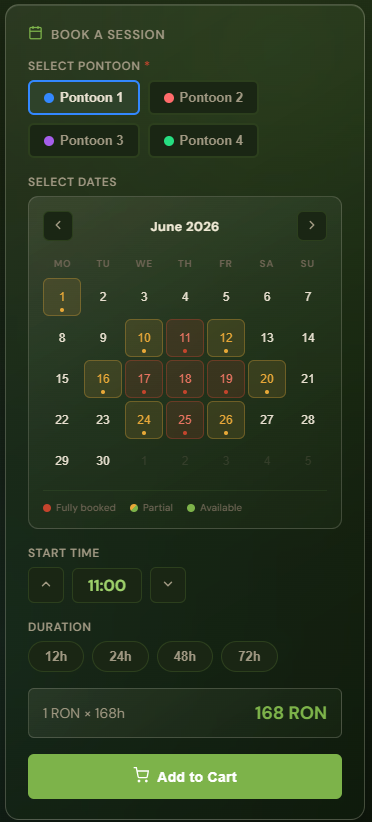
\includegraphics[width=0.45\textwidth]{images/form-calendar.png}
\caption{Calendarul de rezervare cu disponibilitatea pontoanelor și calculul automat al costului}
\label{fig:calendar-rezervare}
\end{figure}

Fluxul de rezervare se finalizează prin plată online sau prin confirmare directă, în funcție de configurația locației. Integrarea cu Stripe este transparentă pentru utilizator: datele de plată sunt completate într-un formular securizat integrat în pagină, fără redirecționare externă. După confirmare, sesiunea apare în istoricul utilizatorului și generează un cod QR asociat rezervării, accesibil direct din aplicație și pregătit pentru verificarea la fața locului.


Modulul de analiză media este accesibil dintr-o secțiune dedicată. Utilizatorul poate încărca o imagine sau un videoclip, iar interfața afișează starea de procesare în timp real printr-un mecanism de polling vizibil. Rezultatele includ speciile detectate, numărul de instanțe identificate și, în cazul videoclipurilor, un rezumat al detecțiilor pe intervale de timp.

\begin{figure}[H]
\centering
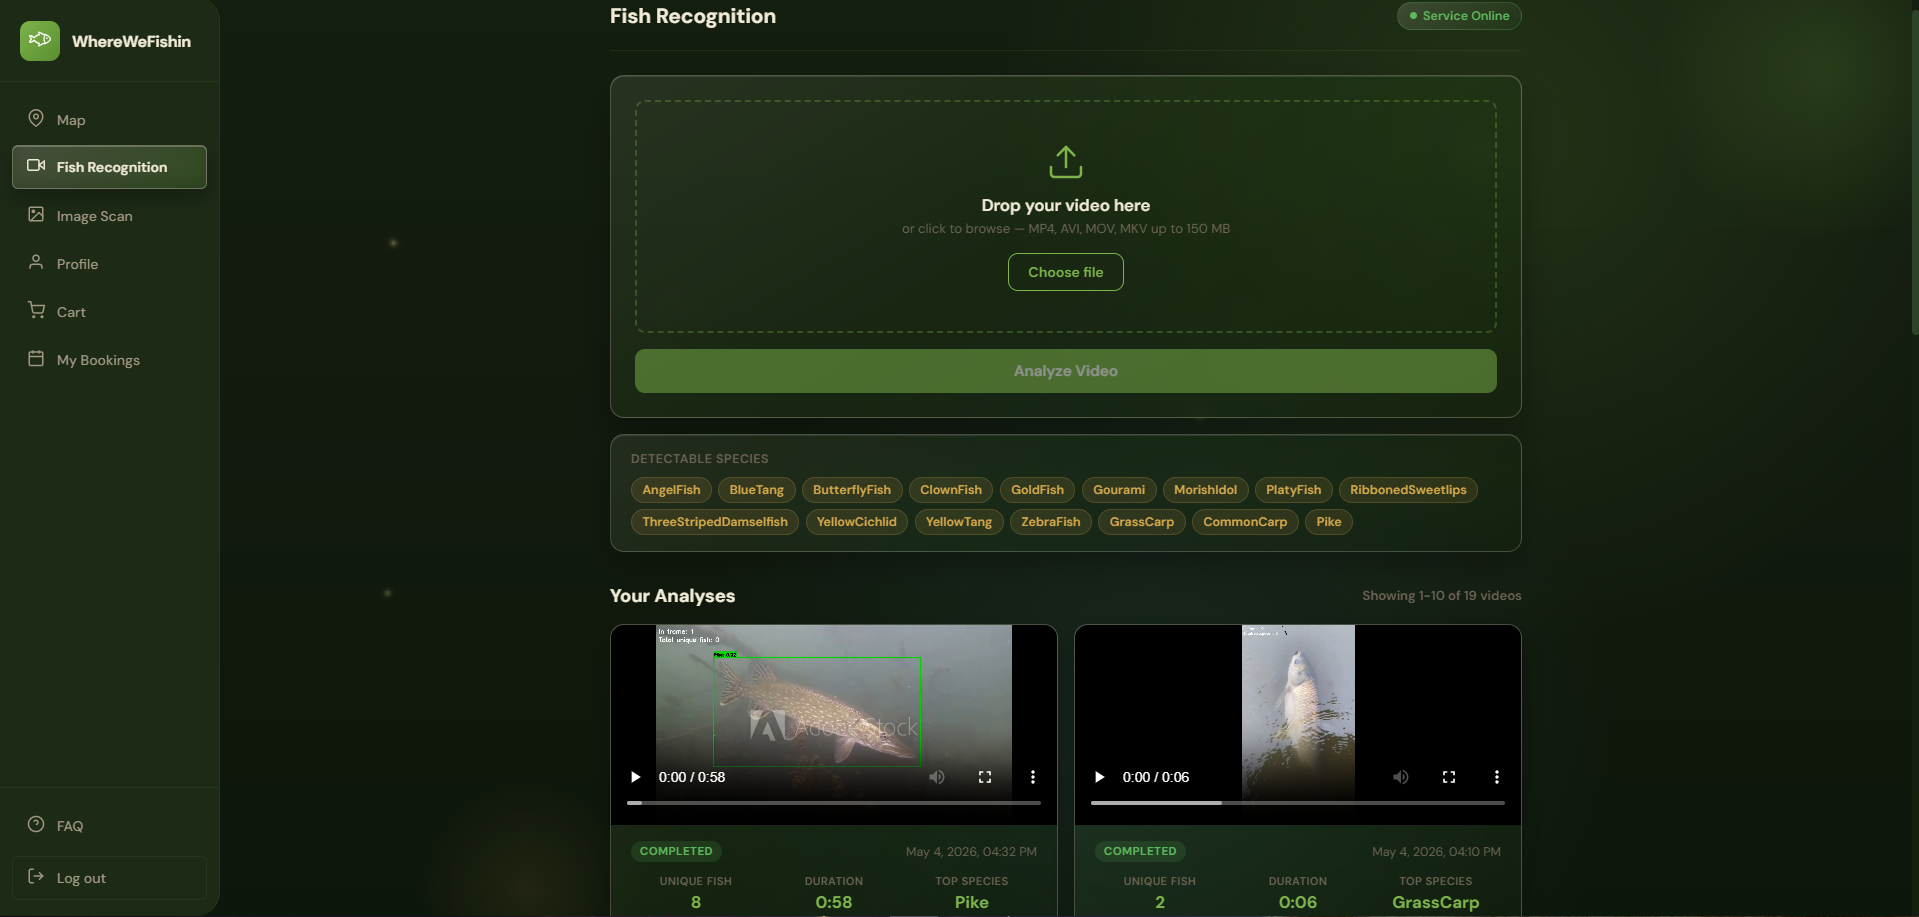
\includegraphics[width=\textwidth]{images/fish-recog.png}
\caption{Pagina de analiză media cu zona de upload, speciile detectabile și istoricul analizelor}
\label{fig:fish-recognition-pagina}
\end{figure}

Componenta este separată intenționat de fluxul de rezervare, pentru a nu complica experiența utilizatorilor care nu doresc să folosească funcția de analiză media.

Secțiunea de profil și istoricul activității oferă utilizatorului o imagine completă a rezervărilor trecute și viitoare, a analizelor media efectuate și a recenziilor lăsate. Această zonă îndeplinește și un rol de trasabilitate: utilizatorul poate oricând verifica detaliile unei rezervări, inclusiv codul QR, fără a depinde de un email de confirmare.

\section{Interfața managerului și dashboard-ul operațional}

Zona managerului este construită în jurul unui dashboard care concentrează informațiile operaționale relevante pentru administrarea unui loc de pescuit. Structura este organizată pe secțiuni distincte: administrarea pontoanelor, gestionarea angajaților, informații despre locație și rezervările active.

Prima secțiune vizibilă la accesarea dashboard-ului este suita de statistici agregate: numărul total de rezervări create, rezervările active în ziua curentă, veniturile cumulate, ratingul mediu al locației și numărul de recenzii primite. Imediat sub statistici, un grafic de bare prezintă distribuția sesiunilor pe zile sau săptămâni, oferind o imagine rapidă a ritmului de activitate. Aceste date permit managerului să evalueze starea locației dintr-o privire, înainte de a intra în secțiunile de detaliu.

Meniul lateral oferă acces direct la subsecțiunile principale: dashboard-ul cu vederea de ansamblu, modulul de administrare a pontoanelor, secțiunea de repopulare cu pești și panoul de setări ale locației. Această organizare separă clar activitățile de monitorizare de cele de administrare propriu-zisă, permițând managerului să comute rapid între contexte fără a pierde starea curentă a paginii. Butonul de reîmprospătare manuală, plasat în partea superioară, permite actualizarea instantanee a statisticilor fără a necesita reîncărcarea întregii pagini, util mai ales în perioadele de trafic ridicat când rezervările noi apar frecvent.

Secțiunea de informații prezintă datele administrative ale locației: tariful orar configurat, numele managerului responsabil și coordonatele geografice. Lista repopulărilor recente, vizibilă în partea inferioară a dashboard-ului, oferă context operațional important pentru manager: dacă o specie a fost recent repopulată, este probabil să atragă mai mulți pescari în zilele următoare. Figura~\ref{fig:dashboard-manager} ilustrează această vedere de ansamblu, cu toate componentele descrise mai sus.

\begin{figure}[H]
\centering
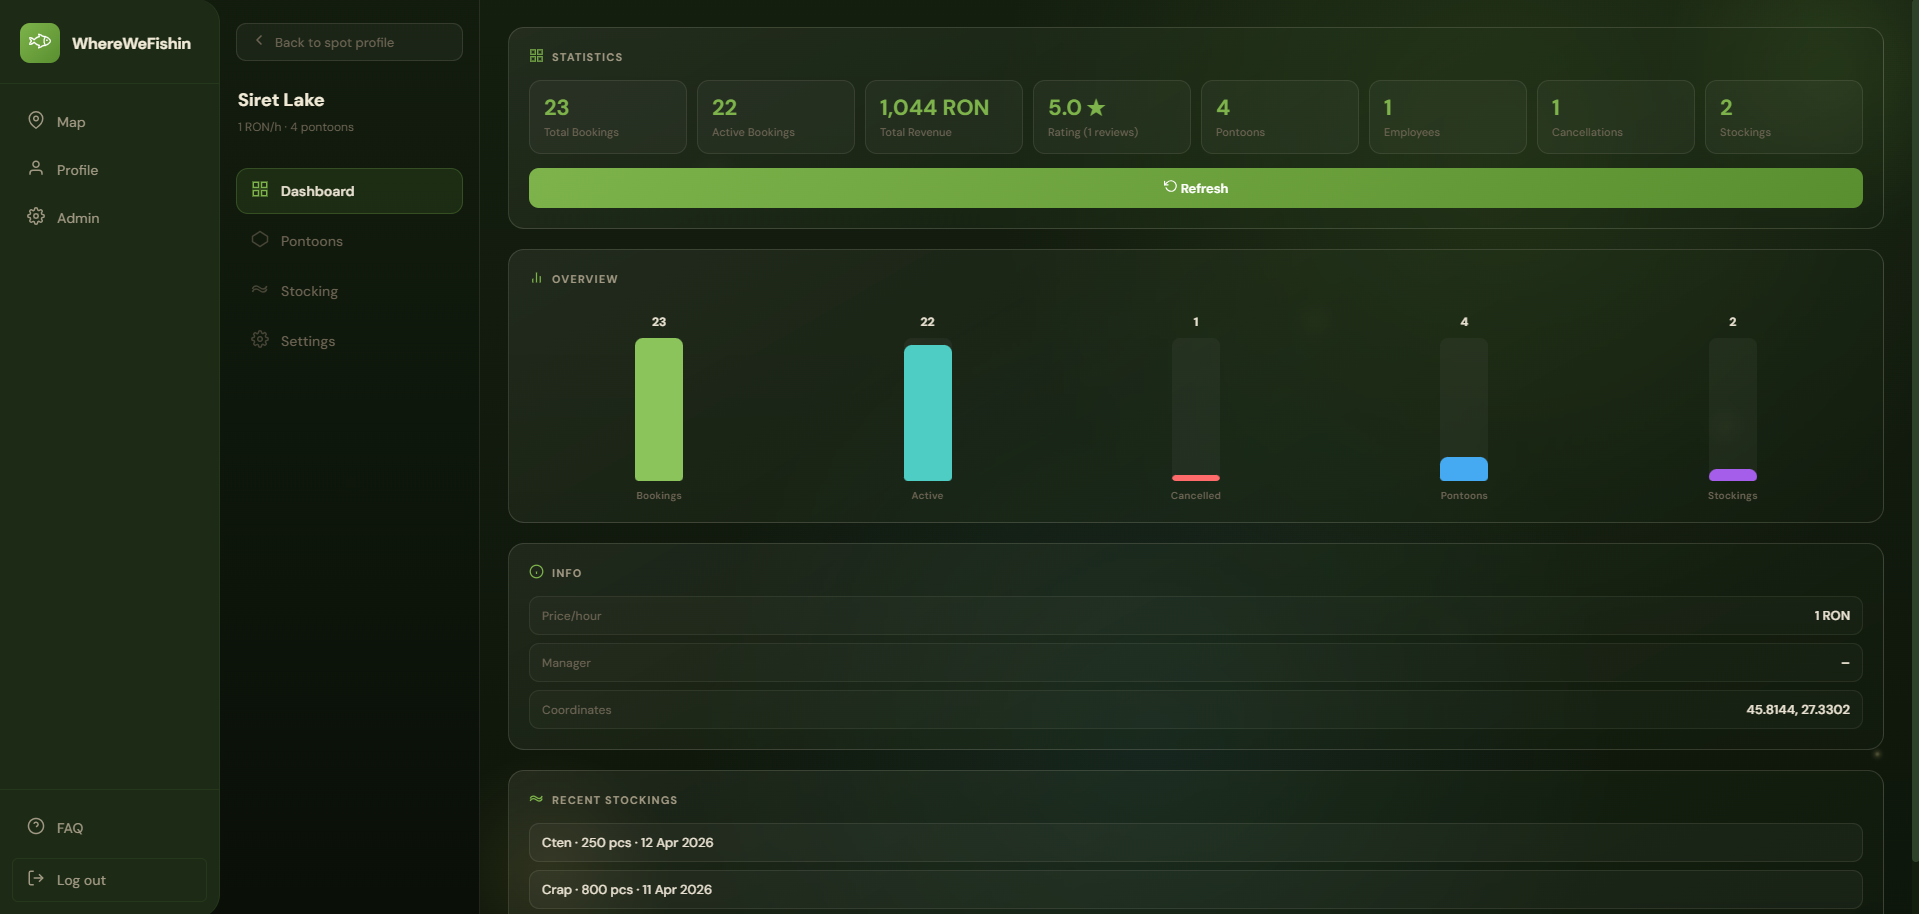
\includegraphics[width=\textwidth]{images/manager-dashboard.png}
\caption{Dashboard-ul managerului cu statistici agregate și graficul de activitate al locației}
\label{fig:dashboard-manager}
\end{figure}

Administrarea pontoanelor utilizează direct harta interactivă: managerul poate adăuga un ponton nou printr-un instrument de desen pe hartă, conturând vizual zona rezervabilă. Coordonatele sunt extrase automat din interacțiunea cu harta, fără a fi nevoie de introducerea manuală a valorilor numerice. Această abordare reduce ambiguitățile și oferă un feedback imediat despre cum va apărea zona în interfața publică, permițând ajustări înainte de salvare.

Gestionarea angajaților permite asocierea utilizatorilor la locație, cu drepturi limitate la operațiile de verificare a sesiunilor. Adăugarea și eliminarea angajaților se face direct din dashboard, fără procese administrative suplimentare. Rezervările active sunt prezentate într-o listă filtrabilă, cu informații despre utilizator, ponton, interval și starea curentă. Managerul poate urmări sesiunile planificate, poate vizualiza confirmările de prezență și poate monitoriza activitatea locației în timp real.

Procesul de aplicare pentru rolul de manager este mediat de un wizard cu mai mulți pași: date descriptive ale locației, poziționare pe hartă și o pagină de revizuire finală înainte de trimitere. Formatul ghidat reduce erorile de completare și permite validarea datelor pe parcurs. Solicitantul poate urmări starea aplicației sale și, în cazul respingerii, poate vizualiza motivul primit de la administrator și poate retrimite cererea cu informațiile corectate.

\section{Experiența angajatului și verificarea prin cod QR}

Angajatul are cel mai restrâns set de funcții, adaptat nevoilor operaționale de la fața locului. Interfața sa principală este componenta de scanare a codului QR, accesibilă direct după autentificare, fără pași intermediari.

Componenta de scanare utilizează camera dispozitivului și procesează codul QR al sesiunii de pescuit. Decodificarea are loc în timp real, cadru cu cadru, printr-o bibliotecă de procesare integrată în browser, fără a trimite imaginea la server. Când codul este identificat, token-ul de rezervare este extras și trimis backend-ului pentru validare: sistemul verifică că sesiunea aparține locației angajatului, că intervalul este activ și că prezența nu a fost deja confirmată. Rezultatul validării apare imediat în interfață, fără navigare sau pași intermediari. Figura~\ref{fig:qr-scanner-angajat} prezintă interfața componentei, cu locația asignată și camera activă.

\begin{figure}[H]
\centering
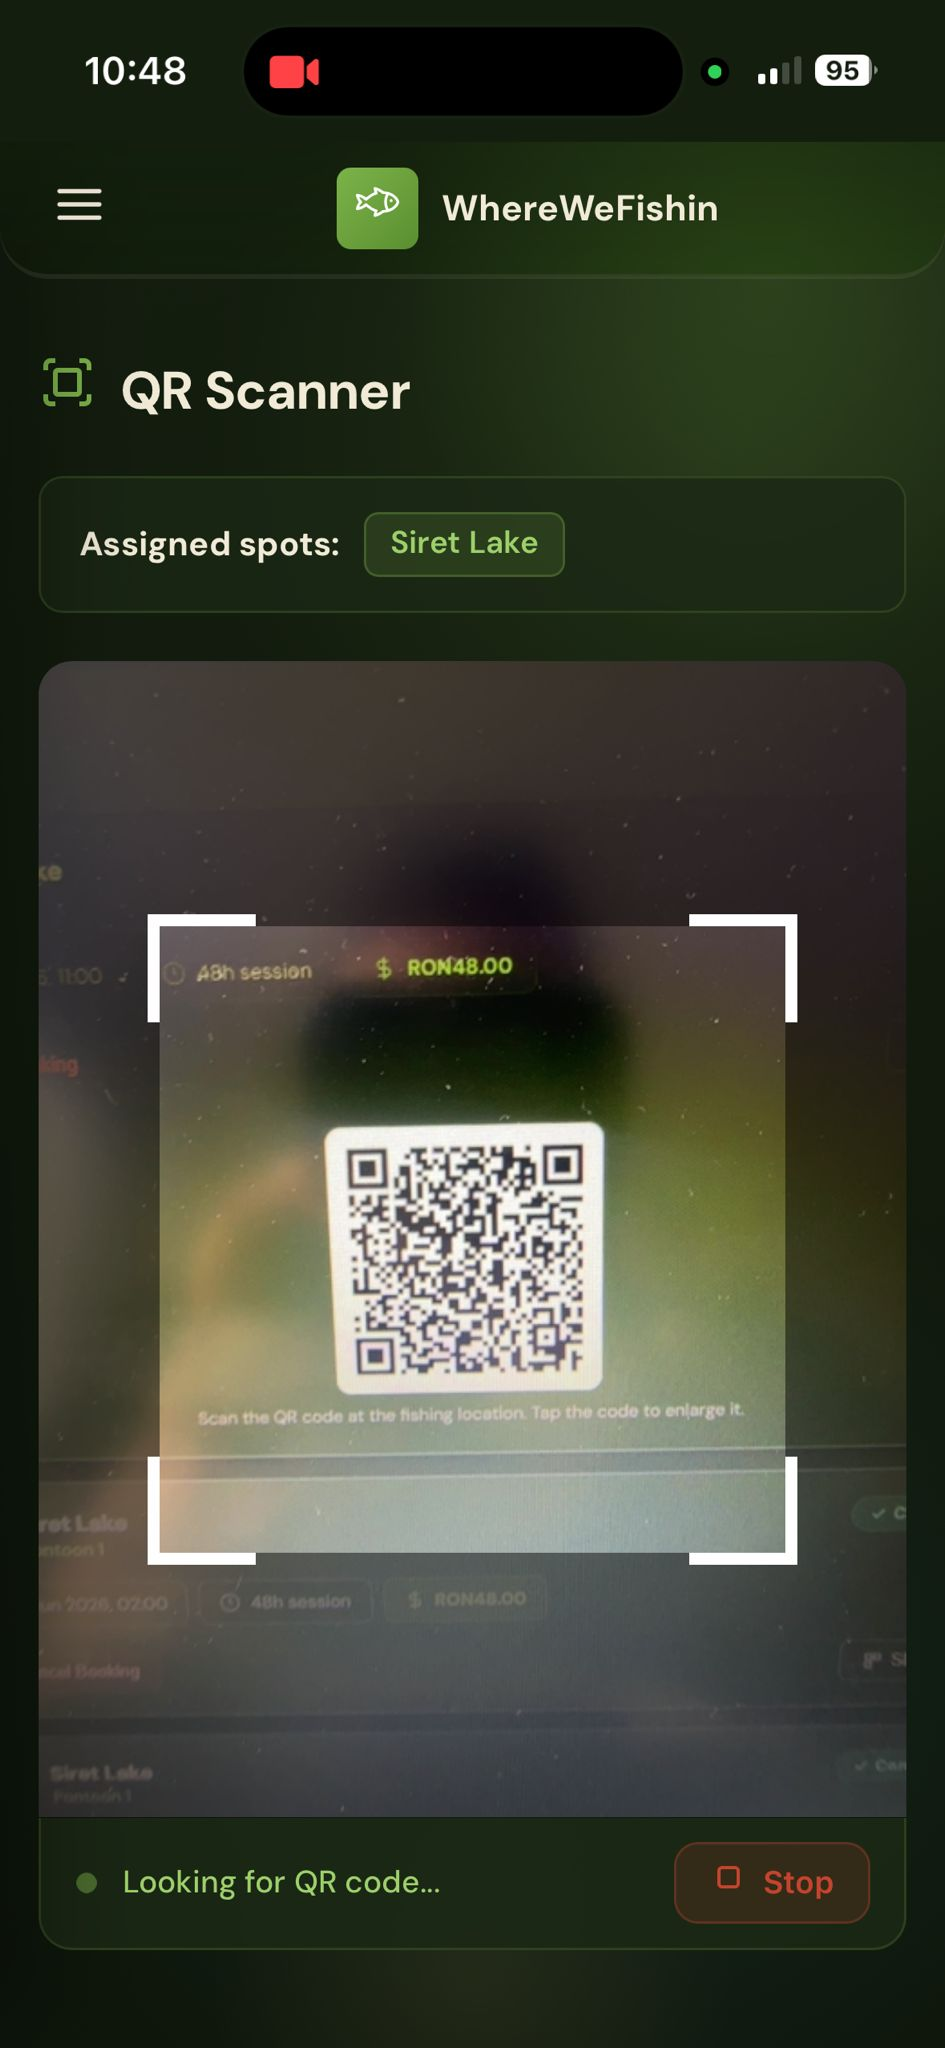
\includegraphics[width=0.45\textwidth]{images/angajat-qrpage.jpeg}
\caption{Interfața de scanare QR a angajatului, cu locația asignată și camera activă}
\label{fig:qr-scanner-angajat}
\end{figure}

Odată identificată sesiunea, interfața afișează detaliile rezervării: utilizatorul, pontonul, intervalul și starea curentă. Dacă sesiunea este validă și în intervalul corect, angajatul confirmă prezența cu o singură acțiune. Dacă există o neconcordanță, de exemplu sesiune expirată, ponton diferit sau cod invalid, interfața afișează un mesaj explicit care descrie problema, fără a bloca complet fluxul.

Această abordare este importantă pentru utilizarea în teren. Angajatul lucrează adesea în condiții care nu permit o interacțiune lungă cu aplicația, de exemplu în aer liber, cu posibilă iluminare variabilă sau conexiune mobilă instabilă. Simplificarea interfeței la funcțiile strict necesare pentru verificare este o decizie deliberată de UX, care prioritizează viteza și claritatea operației în fața complexității vizuale. Angajatul poate verifica o sesiune în câteva secunde, fără a naviga prin meniuri sau a căuta manual rezervarea în liste.

\section{Panoul administrativ}

Administratorul platformei are acces la o zonă separată, cu funcții de supraveghere globală. Principalele secțiuni vizează gestionarea utilizatorilor înregistrați, monitorizarea locurilor de pescuit active și procesarea aplicațiilor pentru rolul de manager.

Fluxul de aprobare a aplicațiilor este direct și bine delimitat: administratorul vede lista cererilor primite, poate accesa detaliile fiecăreia, inclusiv datele descriptive ale locației propuse și informațiile despre solicitant, și ia o decizie de aprobare sau respingere. În cazul respingerii, câmpul de motivație permite transmiterea unui feedback util solicitantului, reducând iterațiile de comunicare. O cerere aprobată transformă automat utilizatorul în manager, creează locul de pescuit în platformă și îl face vizibil pe hartă.

Zona administrativă oferă și o vizualizare de ansamblu a utilizatorilor și locațiilor active. Administratorul poate interveni în cazuri excepționale (suspendarea unui cont sau dezactivarea unei locații) fără a depinde de acțiuni externe. Această funcție de supraveghere nu înlocuiește un instrument dedicat de monitorizare, dar oferă suficiente informații pentru gestionarea curentă a platformei în stadiul actual de dezvoltare.

\section{Gestionarea autentificării și comunicarea cu API-ul}

O aplicație Angular de tip SPA care consumă un API securizat cu JWT trebuie să rezolve mai multe probleme tehnice: stocarea tokenului, atașarea lui la fiecare cerere, protejarea rutelor private și gestionarea expirării sesiunii.

Tokenul JWT primit la autentificare este stocat în \texttt{localStorage}, ceea ce îl face persistent între sesiuni de browser. La fiecare cerere HTTP, un \emph{interceptor} Angular atașează automat header-ul \texttt{Authorization: Bearer <token>} la toate cererile destinate API-ului. Interceptorul verifică prezența tokenului și îl adaugă fără nicio intervenție explicită în componentele care inițiază cererile. Dacă API-ul returnează HTTP 401, interceptorul poate declanșa delogarea automată și redirecționarea spre pagina de autentificare.

Protecția rutelor private este realizată prin \emph{route guards}. Fiecare zonă funcțională, anume dashboard manager, panou angajat și control administrator, are un guard care verifică dacă utilizatorul este autentificat și dacă rolul său corespunde zonei accesate. Dacă nu, Angular redirecționează automat spre o pagină publică, fără a încărca componenta protejată. Această verificare se face pe baza datelor din token, decodate local la nivel de client: validarea criptografică rămâne exclusiv în responsabilitatea backend-ului.

Serviciile Angular pentru comunicarea cu API-ul sunt organizate pe domenii: un serviciu pentru autentificare, unul pentru rezervări, unul pentru locuri de pescuit și unul pentru analiza media. Fiecare serviciu expune metode tipizate care returnează \texttt{Observable<T>}, permițând componentelor să se aboneze la răspunsuri și să gestioneze stările de încărcare, succes și eroare în mod declarativ. Tiparea statică oferită de TypeScript \citep{typescript} ajută la detectarea erorilor de contract HTTP la momentul compilării, înainte ca acestea să producă probleme în execuție. Această arhitectură facilitează și testarea unitară a logicii de business din frontend, izolat de comunicarea HTTP.

\section{Adaptabilitate și considerații de utilizare mobilă}

Interfața a fost construită cu atenție la comportamentul pe ecrane de dimensiuni diferite. Componentele principale (harta, formularele, listele de rezervări și modulele de analiză media) sunt responsabile și se adaptează la rezoluțiile uzuale ale dispozitivelor mobile și desktop. Acest aspect este important mai ales pentru angajați și utilizatori care accesează aplicația de pe telefon în timp ce se află la locație.

Componenta de scanare QR, utilizată în principal pe dispozitive mobile, a beneficiat de o atenție specială în ceea ce privește toleranța la erori. Implementarea tratează variații ale structurii datelor din cod și gestionează situațiile în care camera nu identifică imediat codul, fără a întrerupe fluxul angajatului. Paginarea listelor de rezultate media și încărcarea întârziată a elementelor video contribuie la o experiență mai fluidă pe conexiuni cu lățime de bandă limitată.

Navigarea pe dispozitive mici a impus și adaptarea meniului și a zonelor de acțiune: elementele interactive au dimensiuni suficiente pentru interacțiune tactilă, iar structura paginilor evită derularea excesivă. Interfața nu implementează funcționalitate offline completă, dar arhitectura sa modulară, bazată pe componente standalone Angular, oferă o bază bună pentru extinderea ulterioară în direcția unui comportament de tip PWA.

\section{Sinteza capitolului}

Interfața WhereWeFishin reflectă structura multi-rol a platformei și prioritizează claritatea față de complexitatea vizuală. Fiecare tip de utilizator are o zonă proprie, cu funcțiile necesare activității sale, fără a fi expus la elemente irelevante. Deciziile de UX au urmărit susținerea fluxurilor reale de utilizare: de la explorarea unui loc de pescuit pe hartă și finalizarea unei rezervări, până la analiza media asistată de inteligență artificială și verificarea prezenței pe teren prin cod QR. Feedback-ul clar pentru operațiile asincrone și adaptabilitatea la dispozitive mobile completează experiența, asigurând o platformă utilizabilă în scenarii variate de acces și context.
